\chapter{Background}
\label{chap:bg}
This chapter is divided into two sections. The first one, \ref{sec:ThB} Theoretical Background,
describes a simple CPU architecture which focuses on the parts used
for executing memory instruction, i.e., stores. It is followed by an introduction of
the three state-of-the-art prefetching strategies. Section \ref{sec:siminf}  goes through the
workflow of this thesis and introduce the tools that are used, modified or created, as
well as how they are combined.
\THsec{Theoretical Background}{ThB}

\THsub{A theoretical Architecture}{TA}
\begin{figure}[h]
\centering
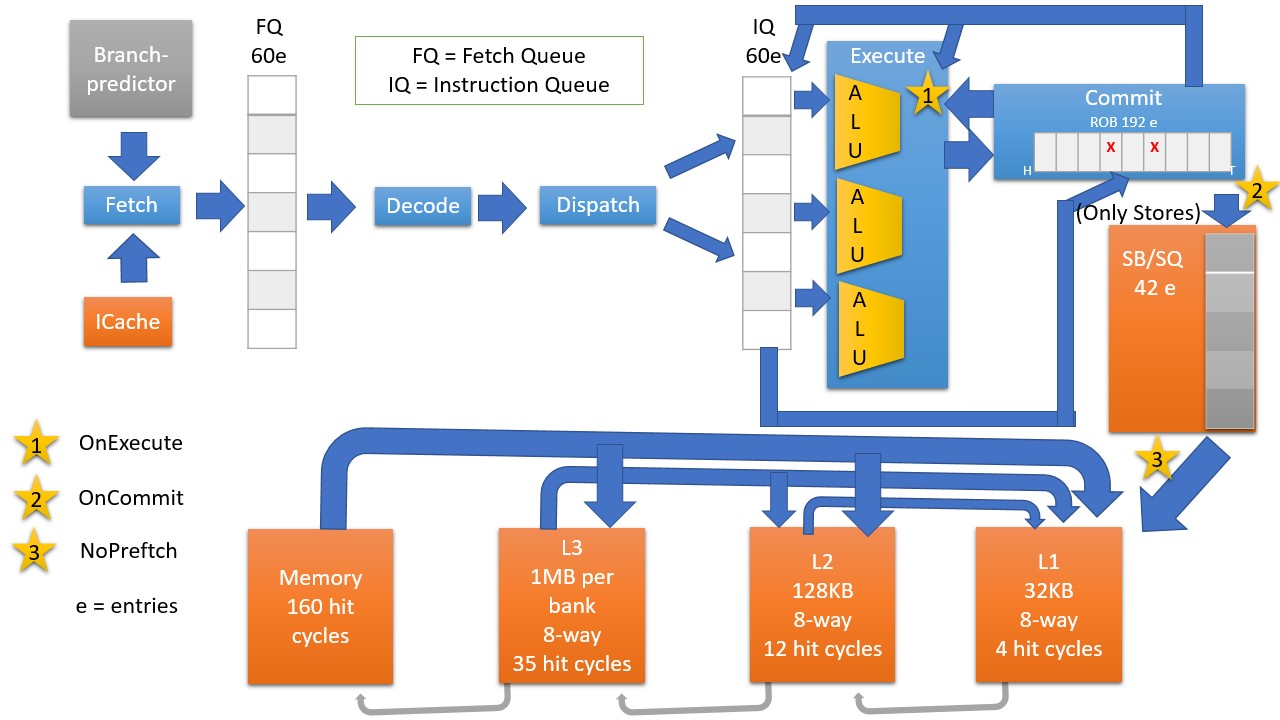
\includegraphics[width=12cm]{figure/thoeratical-arc.jpg}
\caption{Our architecture}
\label{img:arc}
\end{figure}
The image \ref{img:arc} shows architecture in use. This image symbolizes almost all
the features and parts of the CPU that are going to be discussed and analyzed from different
perspectives. If there is a picture that you should keep in mind when reading
this report, this would be it. The stars symbolize where a prefetch is issued for the three state-of-the-art store prefetch policies evaluated in this thesis (section \ref{subsec:GPP}). The structure is the one used for the simulated CPU (see section \ref{sec:arc}). In modern CPU’s there is often more than one core which all have a processor pipeline with several stages. The pipeline is split into stages to increase the throughput of executed instructions. One can compare it with a car factory where the cars travel on a conveyor belt through different stations and
at each station, something is installed within the car, i.e., seats, wheels or the engine.
\\ \\
The simulated CPU has a seven stage pipeline (for simplicity Decode and Allocation is here combined). Some key parts of the CPU are introduced while covering these stages. One thing to mention before moving
on is that the CPU executes instructions out of order but with the promise that the effect
is always like as if the instruction executed in order.
 \\ \\

\THstage{Fetch}
 A new instruction (see \ref{sec:trace}) is added to the processor. In the most common case the next instruction is brought in from the \THnewWord{I-cache} (Instruction cache). I-cache is a \THnewWord{cache} that holds the instructions to be executed shortly, caches will covered in \ref{subsubsec:memcache}. The CPU has a \THnewWord{PC} (program counter) which keeps track of the address of the current instruction fetched. When fetching the next instruction, the PC increments by the length of the current instruction. Different loops are used in programming, and a loop tells us if we should go back to the beginning of the loop body or if the loop should terminate and the lines below it should execute. A CPU cannot, for example, execute C code directly, it needs to compile first. A compilation is a translation from code to instructions within the instructions set (see \ref{sec:trace}) that are supported by the CPU in question. A loop is compiled to a branch instruction which has a target instruction
address
and the condition to be satisfied if the branch is taken (take one more lap in the
loop). The problem is that we want to continue to bring in new instructions before
the condition is computed, but which instructions are next? Here
the \THnewWord{Branch predictor} come to use since it predicts the outcome of a branch and makes the CPU able to load instructions based on that prediction. If a branch is predicted to be taken the PC is set to the branch target address. If a prediction turns out to be wrong, the CPU has to remove the work and all the side effects produced by the wrongly executed instructions. Fetched instructions are placed in the Fetch queue (FQ) (our has 60 entries).
\THstage{Decode (and Allocation)}
 The instruction (from the instruction queue) will be interpreted here. In the Allocation phase recurses, like entries in the: Issue queue (IQ), Reorder buffer (ROB), and Store buffer (SB) are received~\cite{CPUbook}. The two later buffers are introduced later on.
\THstage{Dispatch}
 In this stage, we take care of dependencies. If adding two numbers and then multiply the result with a third number, then the addition has to be finished before the multiplication can be executed. Thus the multiplication has a dependency on the addition. If the result of the multiplication have to be stored, then the multiplication needs to be computed before the result of it can stored. This gives a dependency between the store and the multiplication. When the dependencies have been worked out, the instructions will be put in the \THnewWord{Instruction queue} (IQ) (which has 60 entries as well).
\THstage{Execute}

Here is the arithmetic computation performed. It takes place in one of the arithmetic logic units (ALUs), for the store instructions this means calculating the memory address. The instructions may be executed out-of-order. 

\THstage{Commit}
Commit is the last step of the pipeline, and it shares the ROB (ReOrdering Buffer),
with 192 entries, with some of the previous stages. This buffer puts the out-of-order executed instructions back into
order. Given the size of the ROB, it is possible to execute up to 191 instructions ahead while waiting for an instruction to finish. When 
 all instructions in a sequence are done, they can leave the pipeline. The {\color{red}x} in figure
\ref{img:arc} illustrates a squashed instruction. If a branch prediction turns out to be wrong,
then we need to squash all the instructions that should never have been executed but
have been based on that incorrect prediction.

 When the addition, with the sum of two number multiplied by a third number, is
 done and the result is added to the ROB, the multiplication instruction in the IQ
(Instruction Queue) gets informed that its dependent instruction is done (the arrow
from ROB to IQ in figure \ref{img:arc}). Finally the arrow from ROB to ALU provides the
result from the addition to the multiplication.

\THstage{Store Buffer (SB)}
 Every instruction takes the path that has been described until now, the path described from beyond this point are only taken by the store instructions. When a store instruction leaves the ROB, it goes to the \THnewWord{store buffer} (also called store queue). The store instruction is now represented by the memory address to be fetched and the data to be stored. The buffer is FIFO-ordered (first in, first out), this means that the first store in the buffer waits for its data to be ready in the L1 cache (see \ref{subsec:TA}) and blocks all stores behind it in the buffer. The store buffer interacts only with the L1 cache.

\THsubsub{Memory and caches}{memcache}
The memory structure (in the bottom of figure \ref{img:arc}) is an essential part when talking about store instructions. Beginning with the main memory that has a storage capacity of some gigabytes, a latency of 160 cycles if a hit, and is located on the motherboard. A cache is a quick and small memory unit that are placed on the CPU chip, in which the data that is likely to be used soon is placed. In this case, we have three caches which are named L1 (32kiB 8-way 4 hit cycles), L2 (128kiB 8-way 12 hit cycles) and L3 (1MB per bank 8-way 35 hit cycles). L stands for level, and the higher the digit, the bigger the cache is and the further away from the core it is located. A bigger cache means that it takes a longer time to find specific data in it. The time is measured in \THnewWord{cycles}, and in every cycle, something can occur in the CPU, i.e., an instruction can be placed in FQ and/or another one can be placed in the ROB. 

If our CPU runs in a frequency of 2.2 GHz, there are:


$$ 2.2 \times 1000^3 = 2.2 \times 10^9 cycle / second$$

Given that one cycles takes:

$$ \frac{1}{2.2 \times 10^9 } = 2.2 \times 10^{-9}s = 2.2ns$$

This gives us that it takes $4 \times 2.2 = 8.8ns$ to retrieve data from the L1 cache. A cache keeps copies of needed data, and the data are saved in different regions
within the cache depending on the data address. The number of ways a cache have,
is the same as the number of data chunks in every address range that can be kept
simultaneously within the cache. The higher number of ways means that it is more
complex to build. The smaller number of ways the higher risk of conflict misses, that
is when the cache runs out of places for data from a specific address range. Our
coaches are all 8-ways which means that a piece of data can be in one of eight places
(if it is in the cache) and that a cache can hold no more than eight data chunks from a
given address range. The I-cache is like another L1 cache that only holds instructions
while the L2 and L3 cache hold both data and instructions. When data loads into
the L1 cache from the main memory, it often loads to all the other caches at the same
time.


\THsub{State-of-the-art prefetch policies}{GPP}
Three approaches were already implemented in the Gems simulator \ref{subsec:GEMs} at the beginning of this thesis and are also covered in the literature. These pros and cons will
be described below based on the architecture introduced in section \ref{subsec:TA}. The ”stars”
mentioned in the paragraph headings are the ones in figure \ref{img:arc}.
\THpar{OnExecute (star 1)}{ONEX}  OnExecute \cite{ONEX} is the earliest and most speculative store
prefetch policy, where the operation to bring data with store permission into the
L1 cache is issued within the execute stage. It ensures that the data arrives in L1
before it is needed, i.e., its instruction in at the head of the store buffer. The downside
is that several events which impact on the data to be prefetched can occur. First, if
the store instruction is affected by a branch, that branch can be mispredicted which
means that energy and space is wasted in the small L1 cache by bringing in unneeded
data. Bringing in data to a cache can cause eviction of other data. When a store
instruction takes first place in the buffer and finds that its data have been evicted
from the L1 cache it has to wait for the data to be brought to the L1 again. It might
take less time since the data can be left in the L2 cache and be brought from it instead
of the main memory.
\\ \\
Given that the prediction is correct there might still be in trouble since when the
prefetch is issued, the instruction has to finish the pipeline and passes through the queue in the buffer. This process might
take a long time. During this time the data can have arrived in the L1 cache and been
evicted due to lack of space. This lack of space is due to more data have been prefetched from the point in
time it arrives in L1 until the instruction is at the head of the store buffer. Prefetching to early
can also become a vulnerability since malicious software can cause a prefetch of illegal data
before the core figures out that it is illegal, and when it does the data have already
been exposed. To conclude, this alternative is the best if nothing goes wrong, but
many things can go wrong.

\THpar{OnCommit (star 2)}{ONCO} In this case, the prefetch is issued in the commit stage (when passing
the store to the store buffer). Unneeded data will not be
prefetched. There is still a possibility that the data will be brought in to the L1 cache and evicted
due to lack of space, as described in the previous paragraph. Prefetching
data on commit might still mean that the instruction may be waiting in the head
of the store buffer. This waiting can, in the worst case, fill up the entire buffer which can stall the
processor, i.e., block it from executing any other instruction. Intel 64 and IA-32 Architecture \cite{ONCO} uses OnCommit. They do not use the name OnCommit, but they
quickly describe a load prefetch with the following sentence: ”Reading for ownership

 and storing the data happens after instruction retirement and follows the order of store
instruction retirement.”. ”Reading for ownership” is the same as prefetch with write
permissions and ”instruction retirement” is another name for instruction commit. To
conclude, OnCommit is the one in the middle between the two extremes, OnExecute
(star 1) and NoPrefetch (star 3).
\THpar{NoPrefetch (star 3)}{NOPF} NoPrefetch does no prefetch, the data will be brought into
the L1 cache when the instruction is in the head of the store buffer. All permission
granted will be needed and not evicted before use. This wastes no energy by bringing
in unneeded data. The downside of this is that every instruction will be blocking the
buffer for a long time waiting on its data to become available in the L1 cache. The
risk for filling up the buffer and stall the processor (see \ref{subsubsec:memcache}) is therefore high.
\\ \\
To conclude: this is the most energy efficient, but also the most time-consuming
trade-off. Upon analyzing the source code of Gem5 \cite{gem5} it was discovered that NoPreftch was the default implemented policy.


\THsec{Simulation infrastructure}{siminf}
Here the tools that have been used for this thesis are covered. The tools that have been modified or created within the work of this master thesis
are to be found in chapter \ref{chap:SettingUpTheTestbed}.
\THsub{Benchmarks}{benchmarks}
To examine how a CPU behaves and how a certain store prefetch policy will work
one has to run, or in this case, simulating the run of a program. These types of programs are often called benchmarks. For this work, the SPEC CPU \textcopyright 2016 industrystandardized benchmark suite \cite{specCpu} was used. It is designed to stress both the CPU and the memory subsystem, and it consists of 55 different benchmark programs that have been used to evaluate different store prefetch policies.
\\ \\
One million instructions from every benchmark are going to be simulated. A warmup of 10\% is used, i.e., the measurements will start after the execution of the first one hundred thousand instructions. A warmup is caused in the beginning of an execution since there will always be a miss in the caches and we do not want that phase to affect the result.
\THsub{Sniper}{sniper}
Sniper is a parallel, high-speed and accurate x86 simulator with support for multicore
according to their website \cite{sniper}. Sniper takes two things as input, a bunch of configurations
that describes the architecture to simulate, and a command line with the call to
the application which we want to simulate, for example, one of the programs in 2.2.1.
Sniper can then produce graphs and other documents that describe and measure the
simulation of the chosen program on the chosen CPU configuration. Two examples
of plots that can be generated are CPI stacks \cite{cpi} and energy stack (bar diagrams with one bar per thread in the program). These bars are divided into different regions
based on the percentages of time or energy spent in that region. The region can be:
Ifetch, mem-l1, mem-l2 or branch.
\THsub{GEMS}{GEMs}
The Wisconsin Multifacet Project at the University of Wisconsin has released a General
Execution-driven Multiprocessor Simulator (GEMS). The simulator is written in
 C/C++ and it is an open-source software. The version used in this work was provided
by my supervisor (Alberto Ros) who had implemented OnCommit and OnExecute,
along with one that he has come up with but not yet published (OnNonBSpeculative).
He has also created support for the changes to the traces in Sniper that was done
during this thesis (see \ref{sec:chSniper}). Support for the policies to be proposed in this work was
implemented based on the received source code. 
GEMS was modified to take a path
to a folder containing traces (like in \ref{sec:trace}), an array of configuration settings (see \ref{sec:conf} and \ref{sec:ThB}) and a path for writing the output stats-file. A stats-file consists of around
2000 lines and is divided into two parts: A configuration part where you find the
information given to GEMS in the configuration array and a Stats part with many
measurements like the number of cycles and the number of accesses to the caches.

